\documentclass[letterpaper,12pt]{article}
\usepackage{tabularx} % extra features for tabular environment
\usepackage{amsmath}  % improve math presentation
\usepackage{float}
\usepackage{pdfpages}
\usepackage{steinmetz}

\usepackage{graphicx} % takes care of graphic including machinery
\graphicspath{ {./figures/} }
\usepackage[margin=1in,letterpaper]{geometry} % decreases margins
\usepackage{cite} % takes care of citations
\usepackage[final]{hyperref} % adds hyper links inside the generated pdf file
\hypersetup{
	colorlinks=true,       % false: boxed links; true: colored links
	linkcolor=blue,        % color of internal links
	citecolor=blue,        % color of links to bibliography
	filecolor=magenta,     % color of file links
	urlcolor =blue         
}




\begin{document}

\title{Experiment 5 Preliminary Work \protect\\ Frequency Response}
\author{Ahmet Akman 2442366 \protect\\}
\date{\today}
\maketitle
\tableofcontents
%\begin{abstract}
%abstract
%\end{abstract}

%\section{Introduction}
\section{Step 1}
The document entitled "Notes on Frequency Response" is read.
\section{Step 2}
\begin{figure}[H]
    \centering
    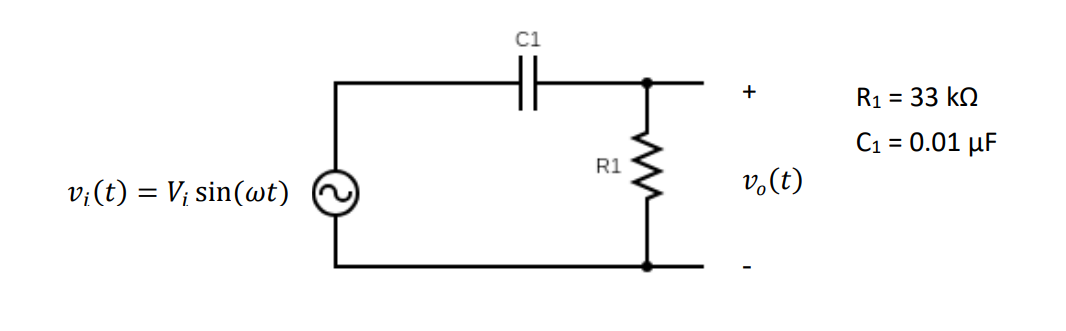
\includegraphics[width=1\textwidth]{RCfilter.png}
    \caption{RC Filter circuit schematic for the step 2}
\end{figure} 
\section{Step 3}
\begin{figure}[H]
    \centering
    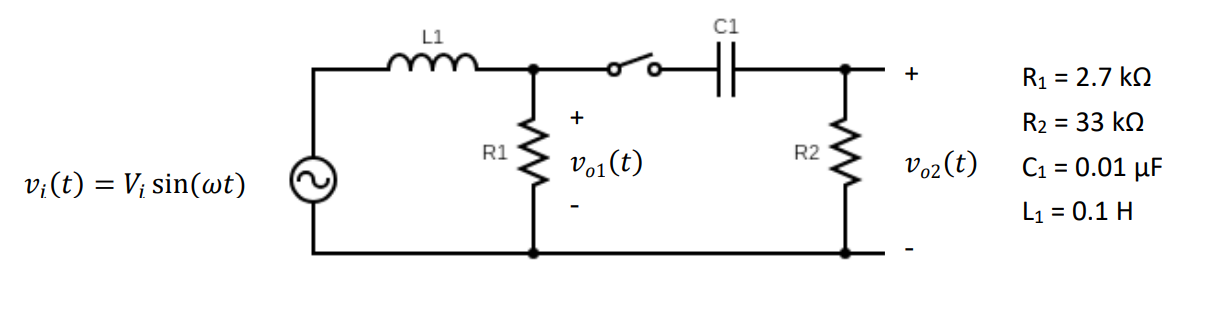
\includegraphics[width=1\textwidth]{lowq.png}
    \caption{Low-Q RC Filter circuit schematic for the step 3}
\end{figure} 
\subsection{a.}
\subsection{b.}

\section{Step 4}
\begin{figure}[H]
    \centering
    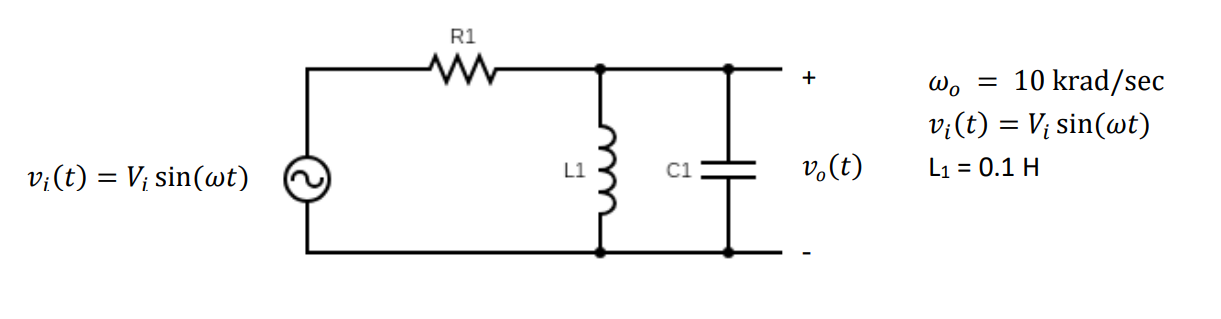
\includegraphics[width=1\textwidth]{highq.png}
    \caption{High-Q RC Filter circuit schematic for the step 4}
\end{figure} 

\subsection{a.}
\subsection{b.}
\subsection{c.}
\begin{figure}[H]
    \centering
    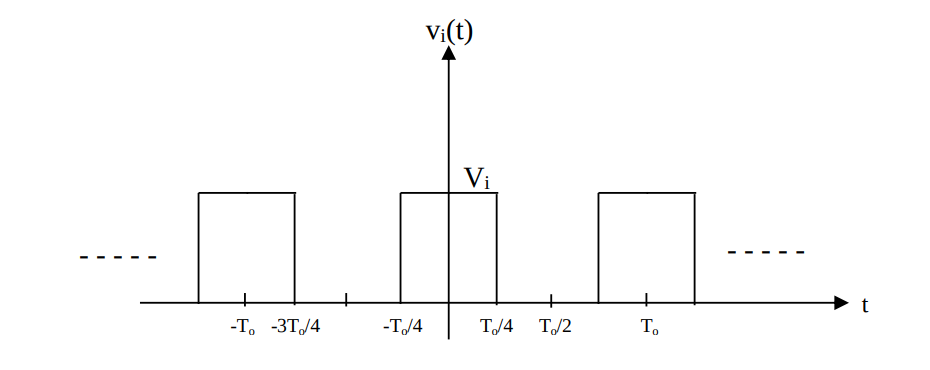
\includegraphics[width=1\textwidth]{RCwaveform.png}
    \caption{Input waveform}
\end{figure} 

\subsection{d.}

\section{Step 5}


\section{Step 6}
In this step necessary simulations are made.

\subsection{a.}
The  circuit given in Figure 1 is simulated in LTSpice simulation environment as given in Figure 5.
\begin{figure}[H]
    \centering
    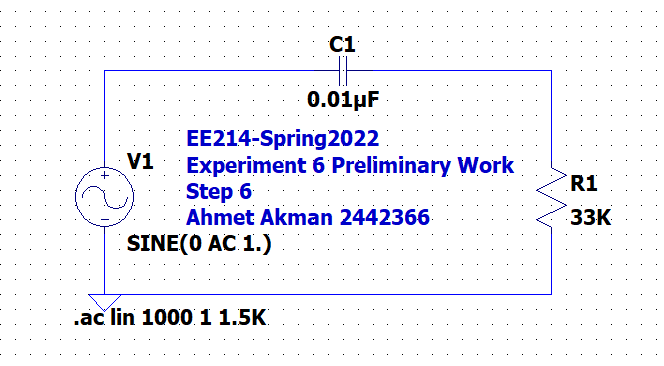
\includegraphics[width=1\textwidth]{6aSim.png}
    \caption{Simulation circuit schematic for the step 6 part a}
\end{figure} 
As a result the plot given in Figure 6 is obtained.
\begin{figure}[H]
    \centering
    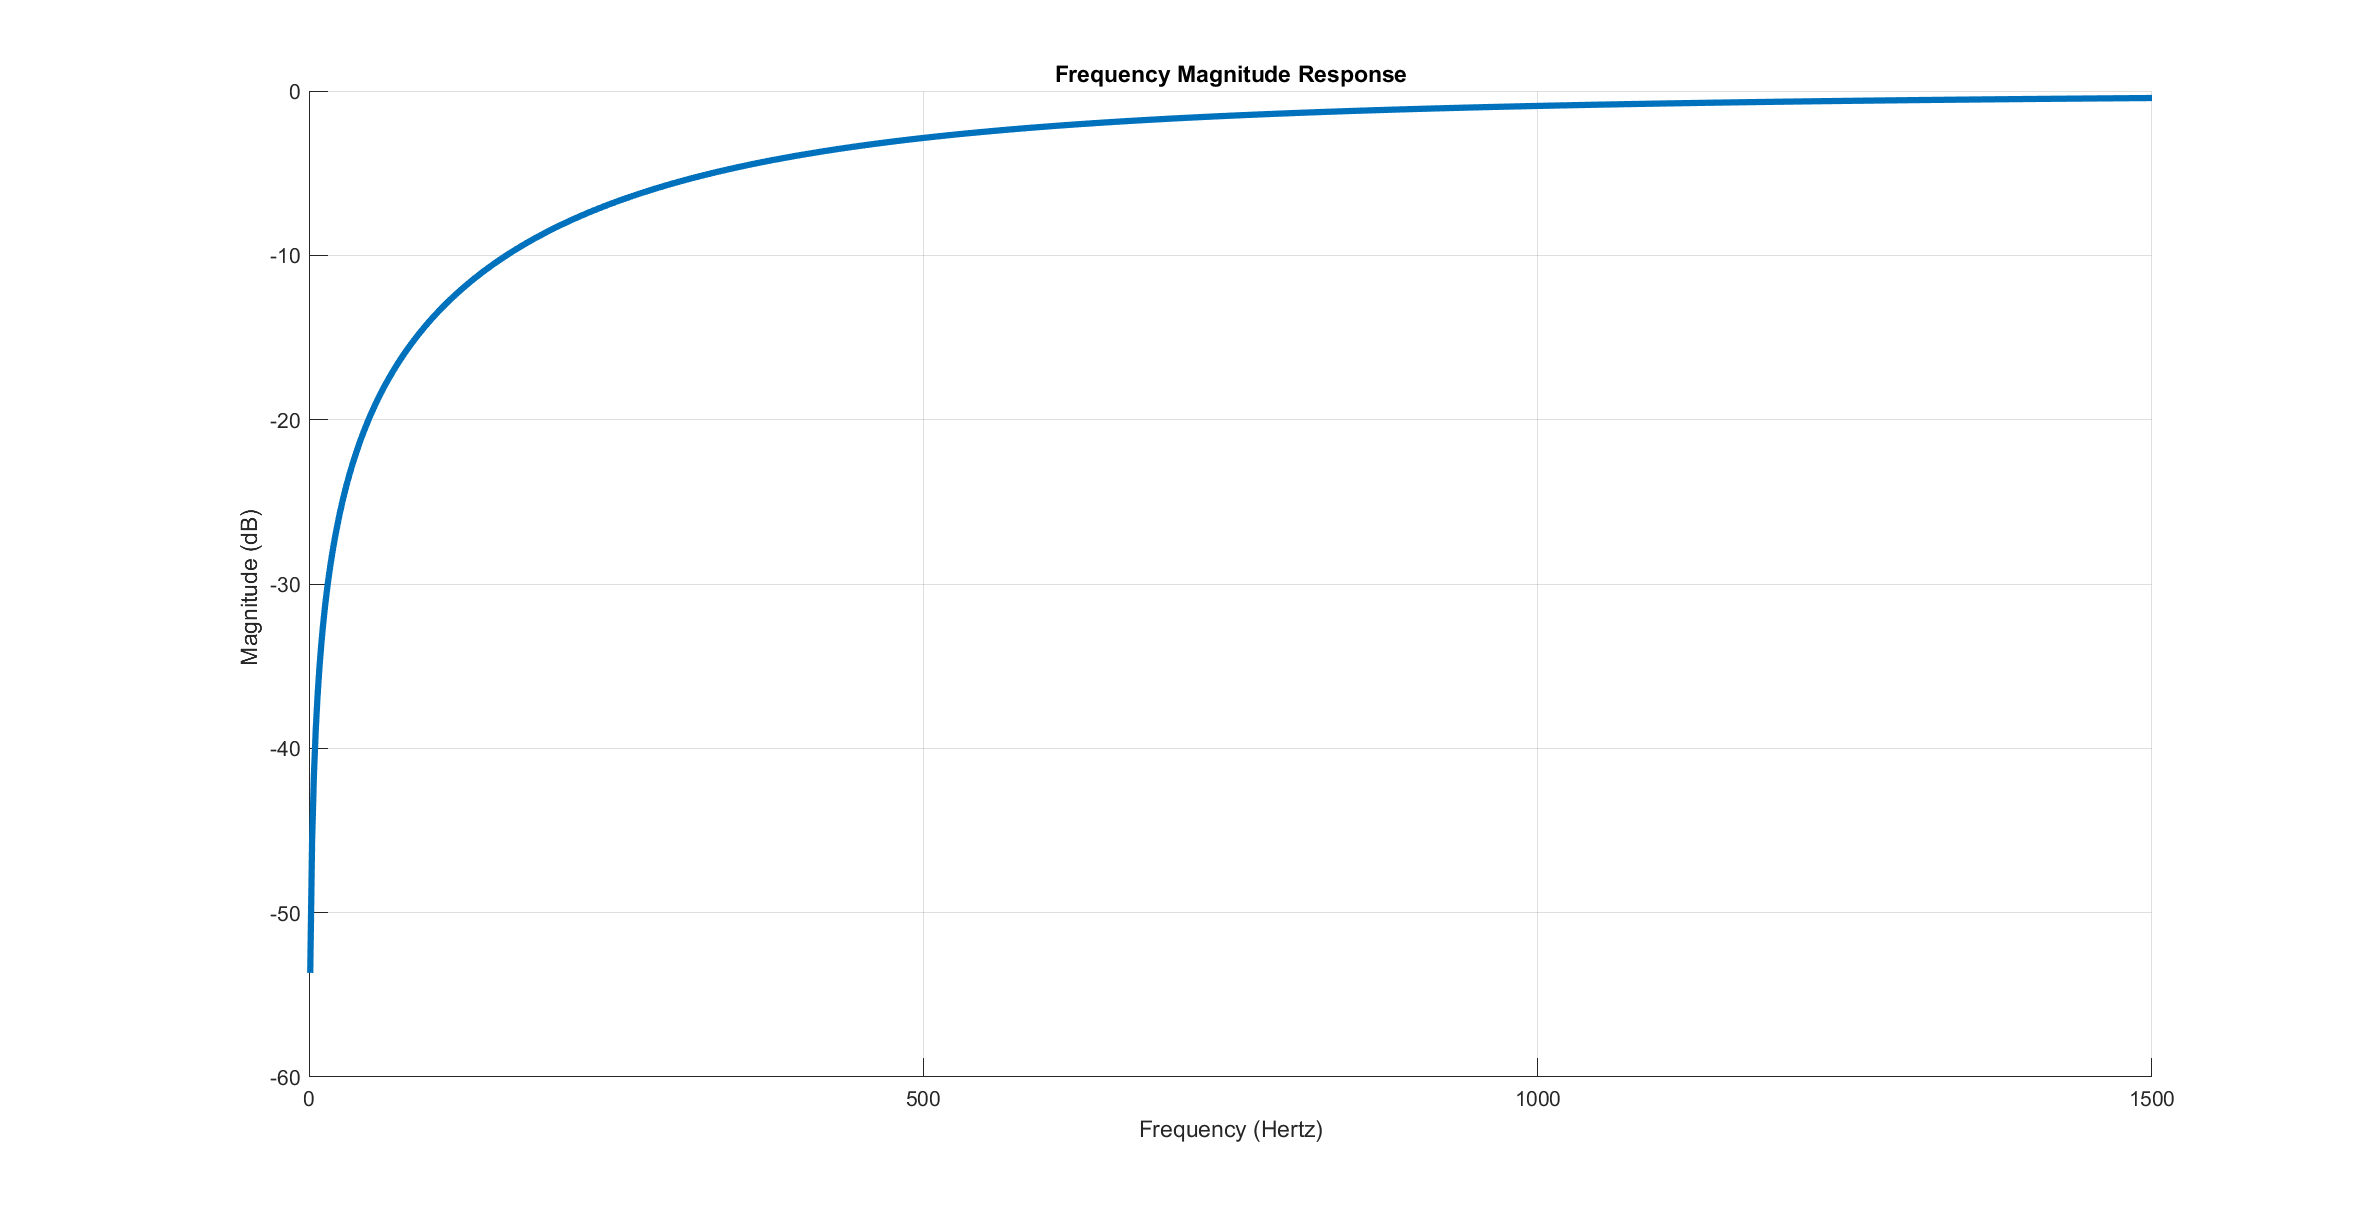
\includegraphics[width=1\textwidth]{6_1.png}
    \caption{Frequency Response of a High Pass Filter}
\end{figure} 


\subsection{b.}
The  circuit given in Figure 2 is simulated in LTSpice simulation environment as given in Figure 7.
\begin{figure}[H]
    \centering
    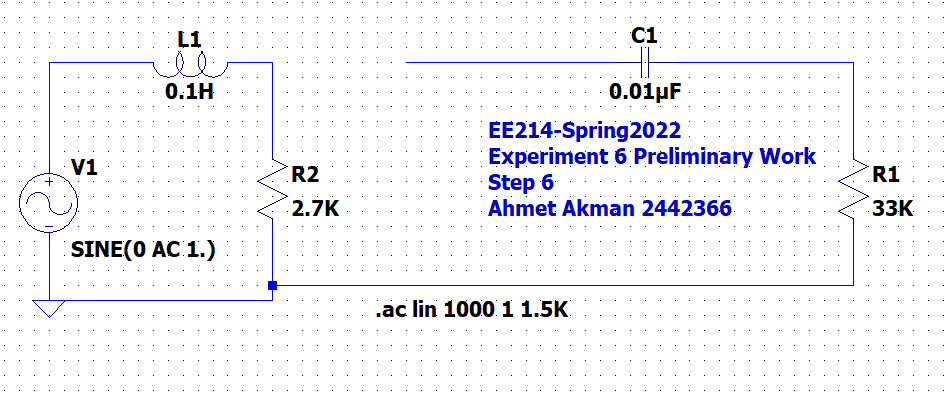
\includegraphics[width=1\textwidth]{6bSim.png}
    \caption{Simulation circuit schematic for the step 6 part b}
\end{figure} 

\subsubsection{i.}
As the switch opened the plot given in Figure 8 is obtained.
\begin{figure}[H]
    \centering
    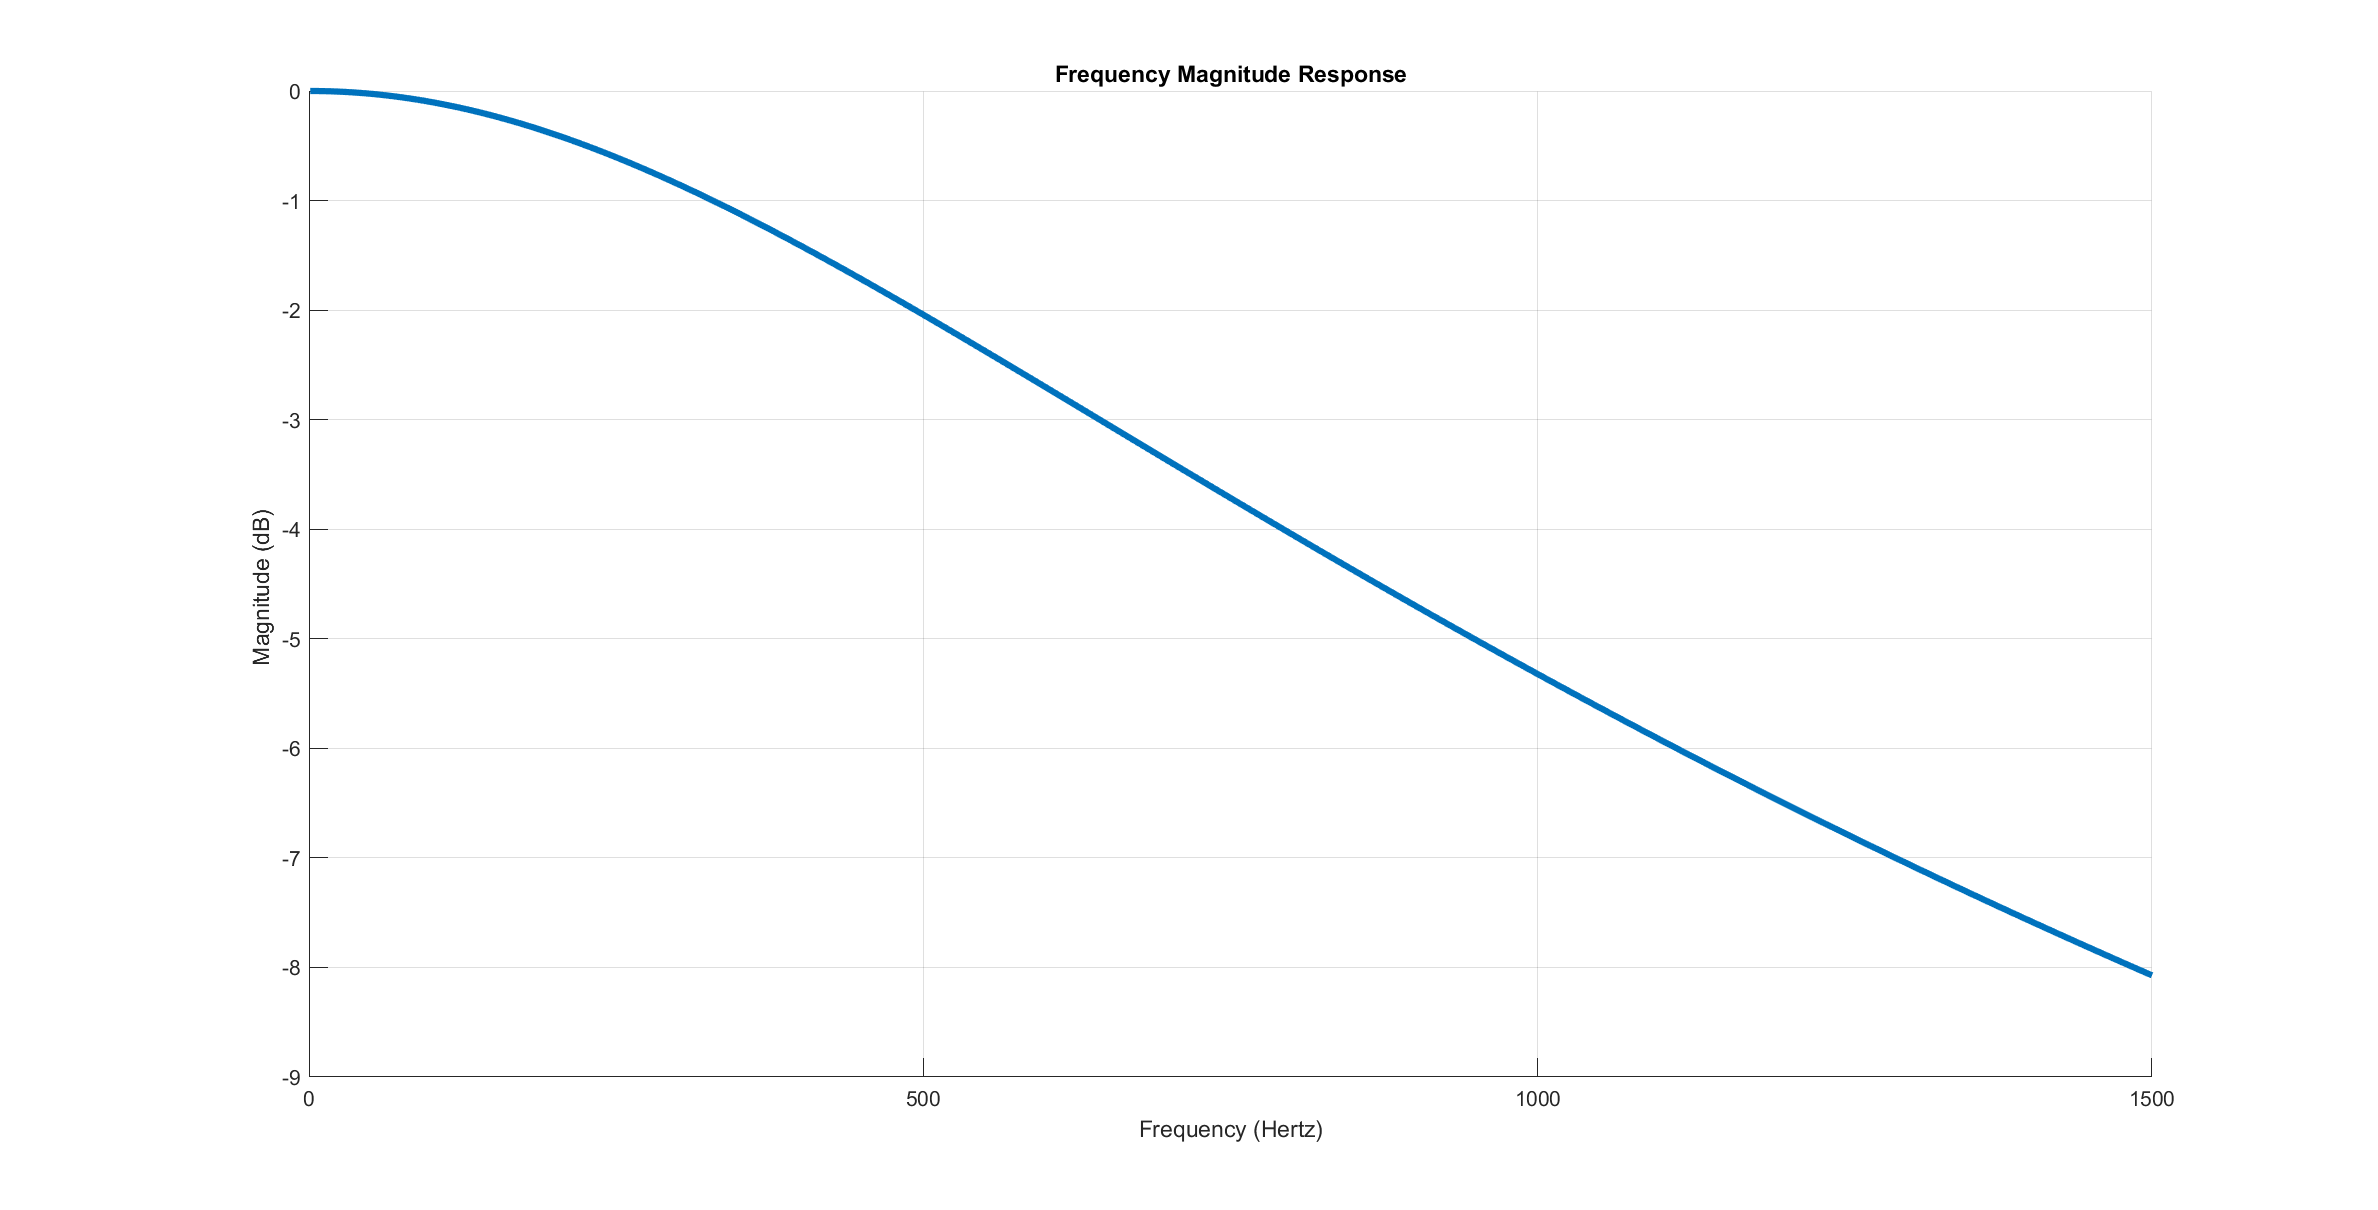
\includegraphics[width=1\textwidth]{6_2_1.png}
    \caption{Frequency Response of a Low Pass Filter}
\end{figure} 


\subsubsection{ii.}
As the switch closed the plot given in Figure 9 is obtained.

\begin{figure}[H]
    \centering
    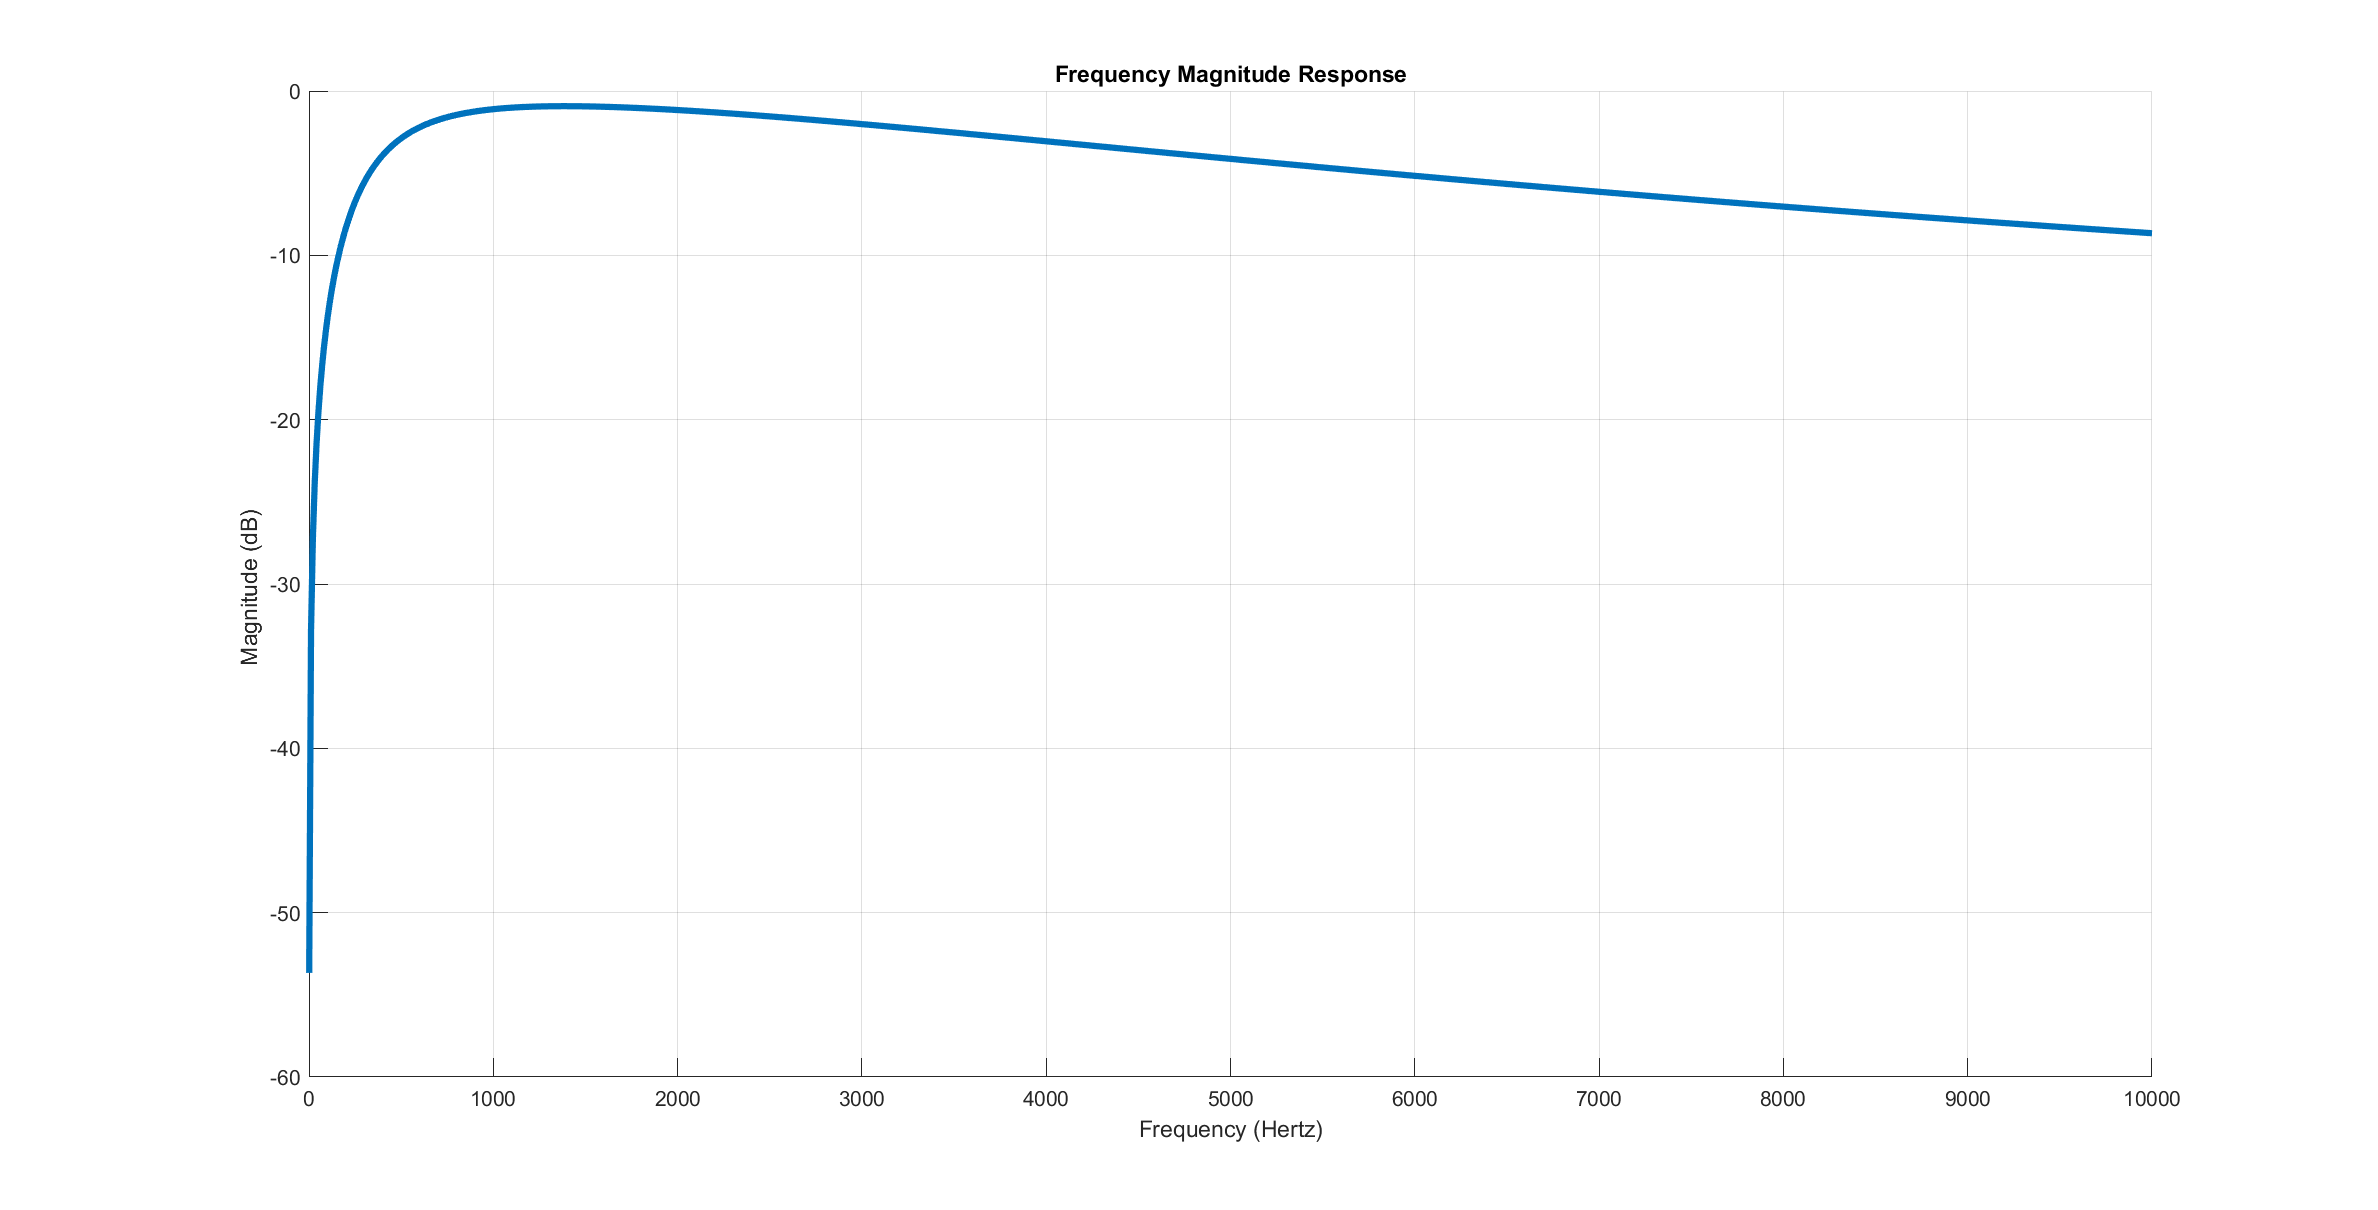
\includegraphics[width=1\textwidth]{6_2_2.png}
    \caption{Frequency Response of a Band Pass Filter}
\end{figure} 

\subsection{c.}
The  circuit given in Figure 3 is simulated in LTSpice simulation environment as given in Figure 10. The capacitor value is fixed as 0.1\(\mu F\)
\begin{figure}[H]
    \centering
    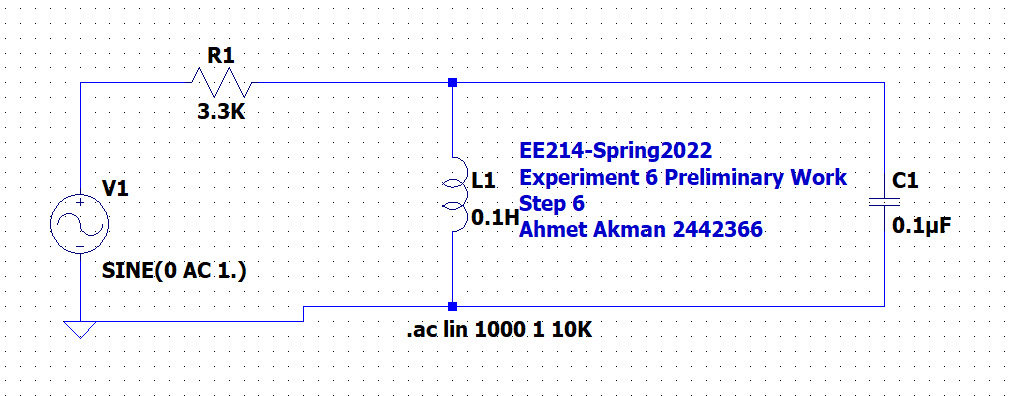
\includegraphics[width=1\textwidth]{6cSim.png}
    \caption{Simulation circuit schematic for the step 6 part c}
\end{figure} 

\subsubsection{i.}
As the resistor value set to 3.3K the plot given in Figure 11 is obtained.
\begin{figure}[H]
    \centering
    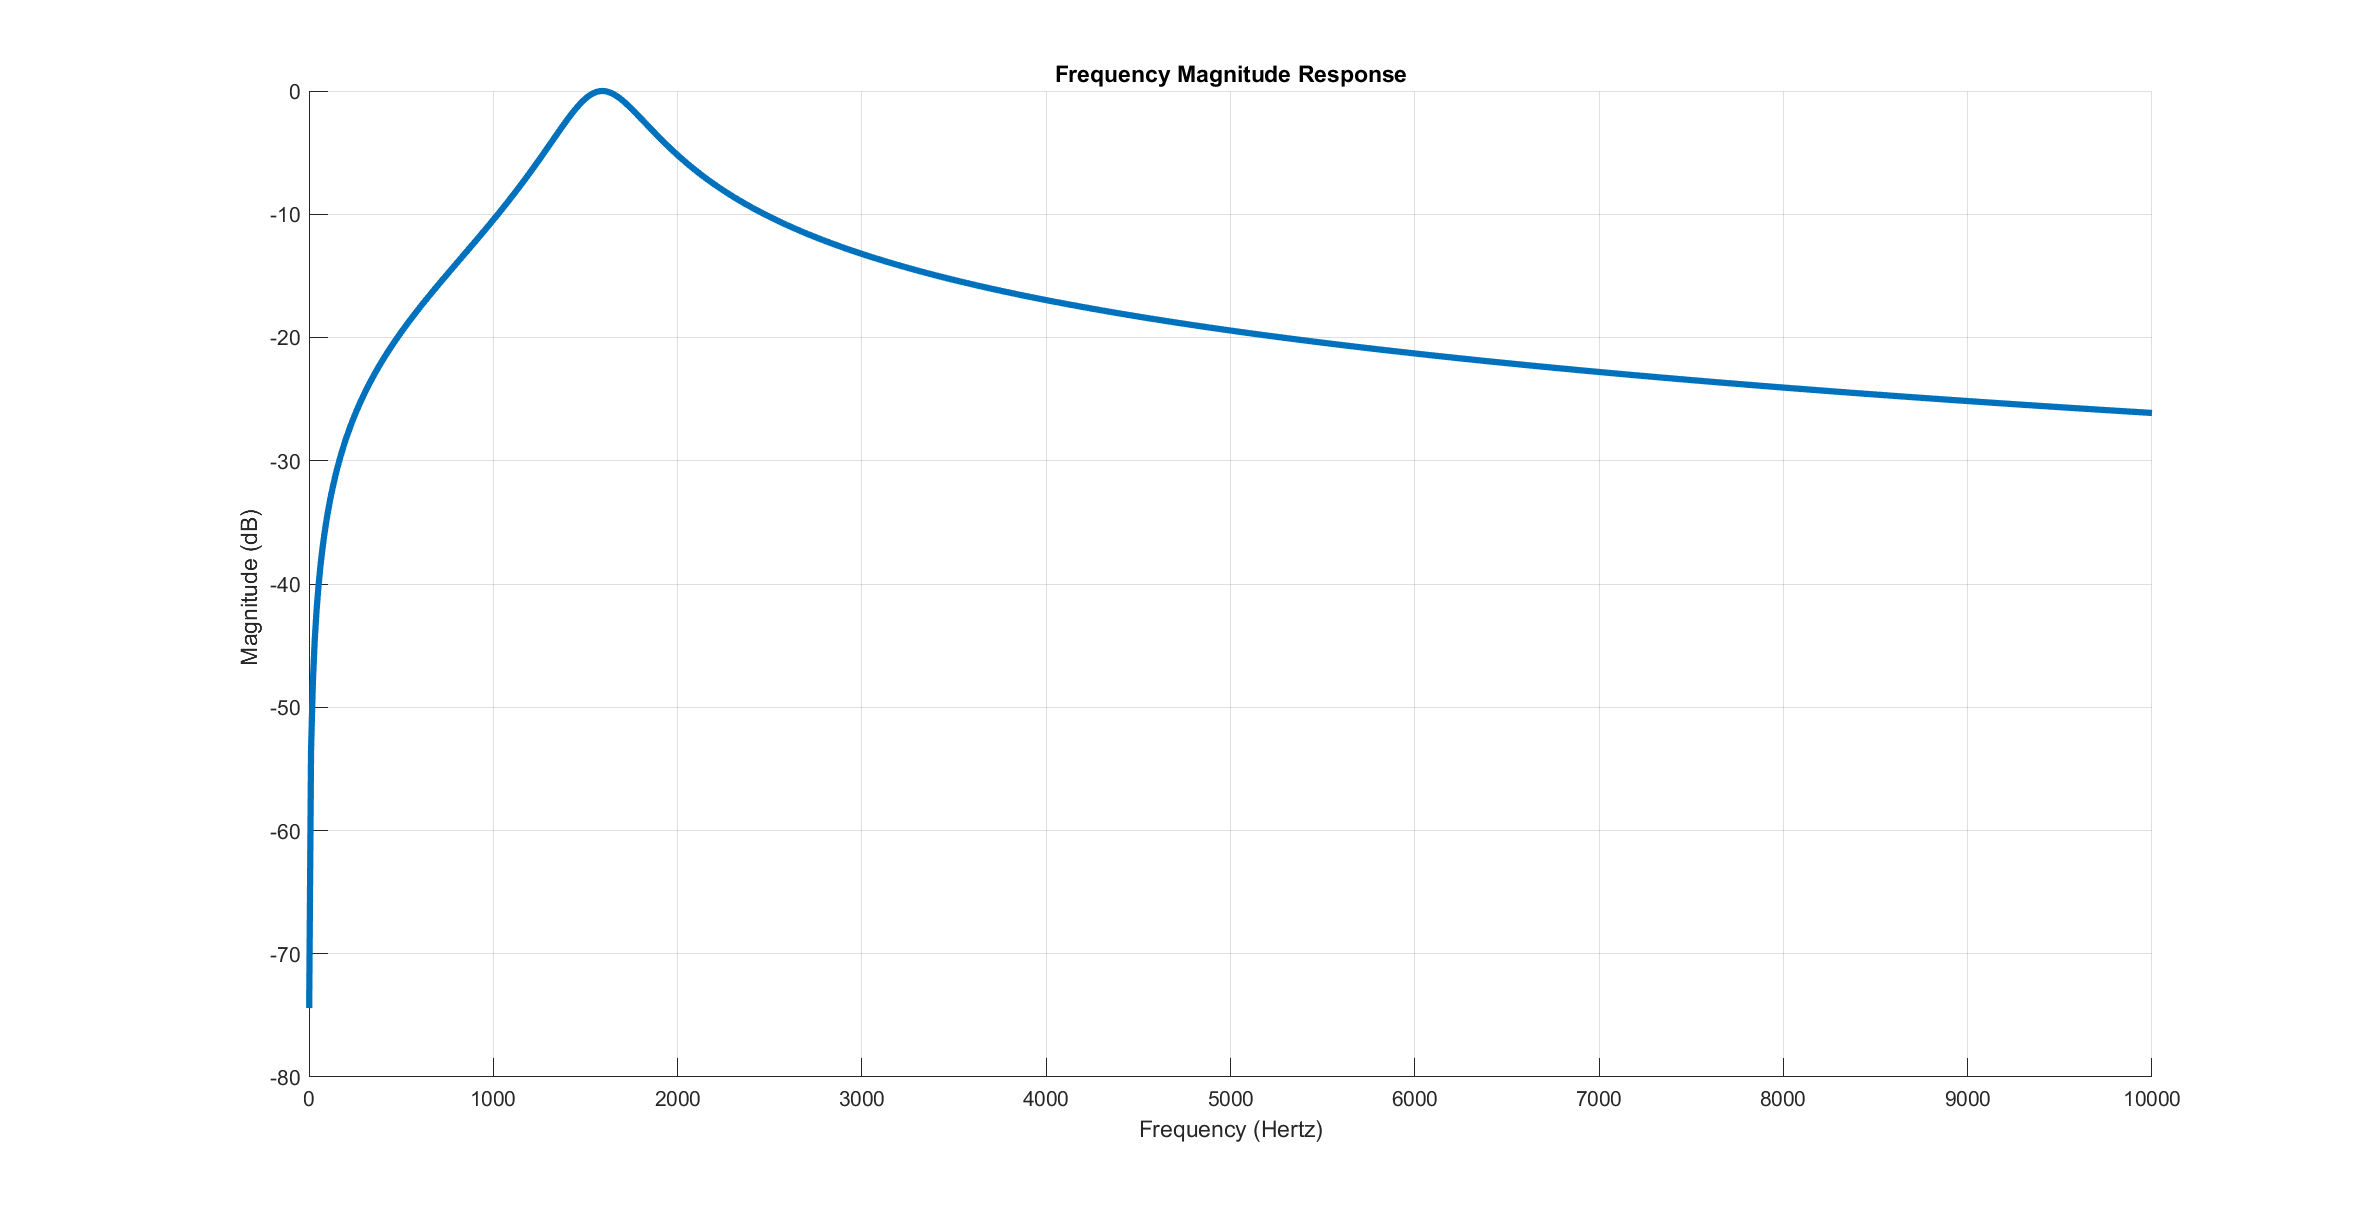
\includegraphics[width=1\textwidth]{6_3_1.png}
    \caption{Frequency Response of a Band Pass Filter}
\end{figure} 

\subsubsection{ii.}
As the resistor value set to 10K the plot given in Figure 12 is obtained.
\begin{figure}[H]
    \centering
    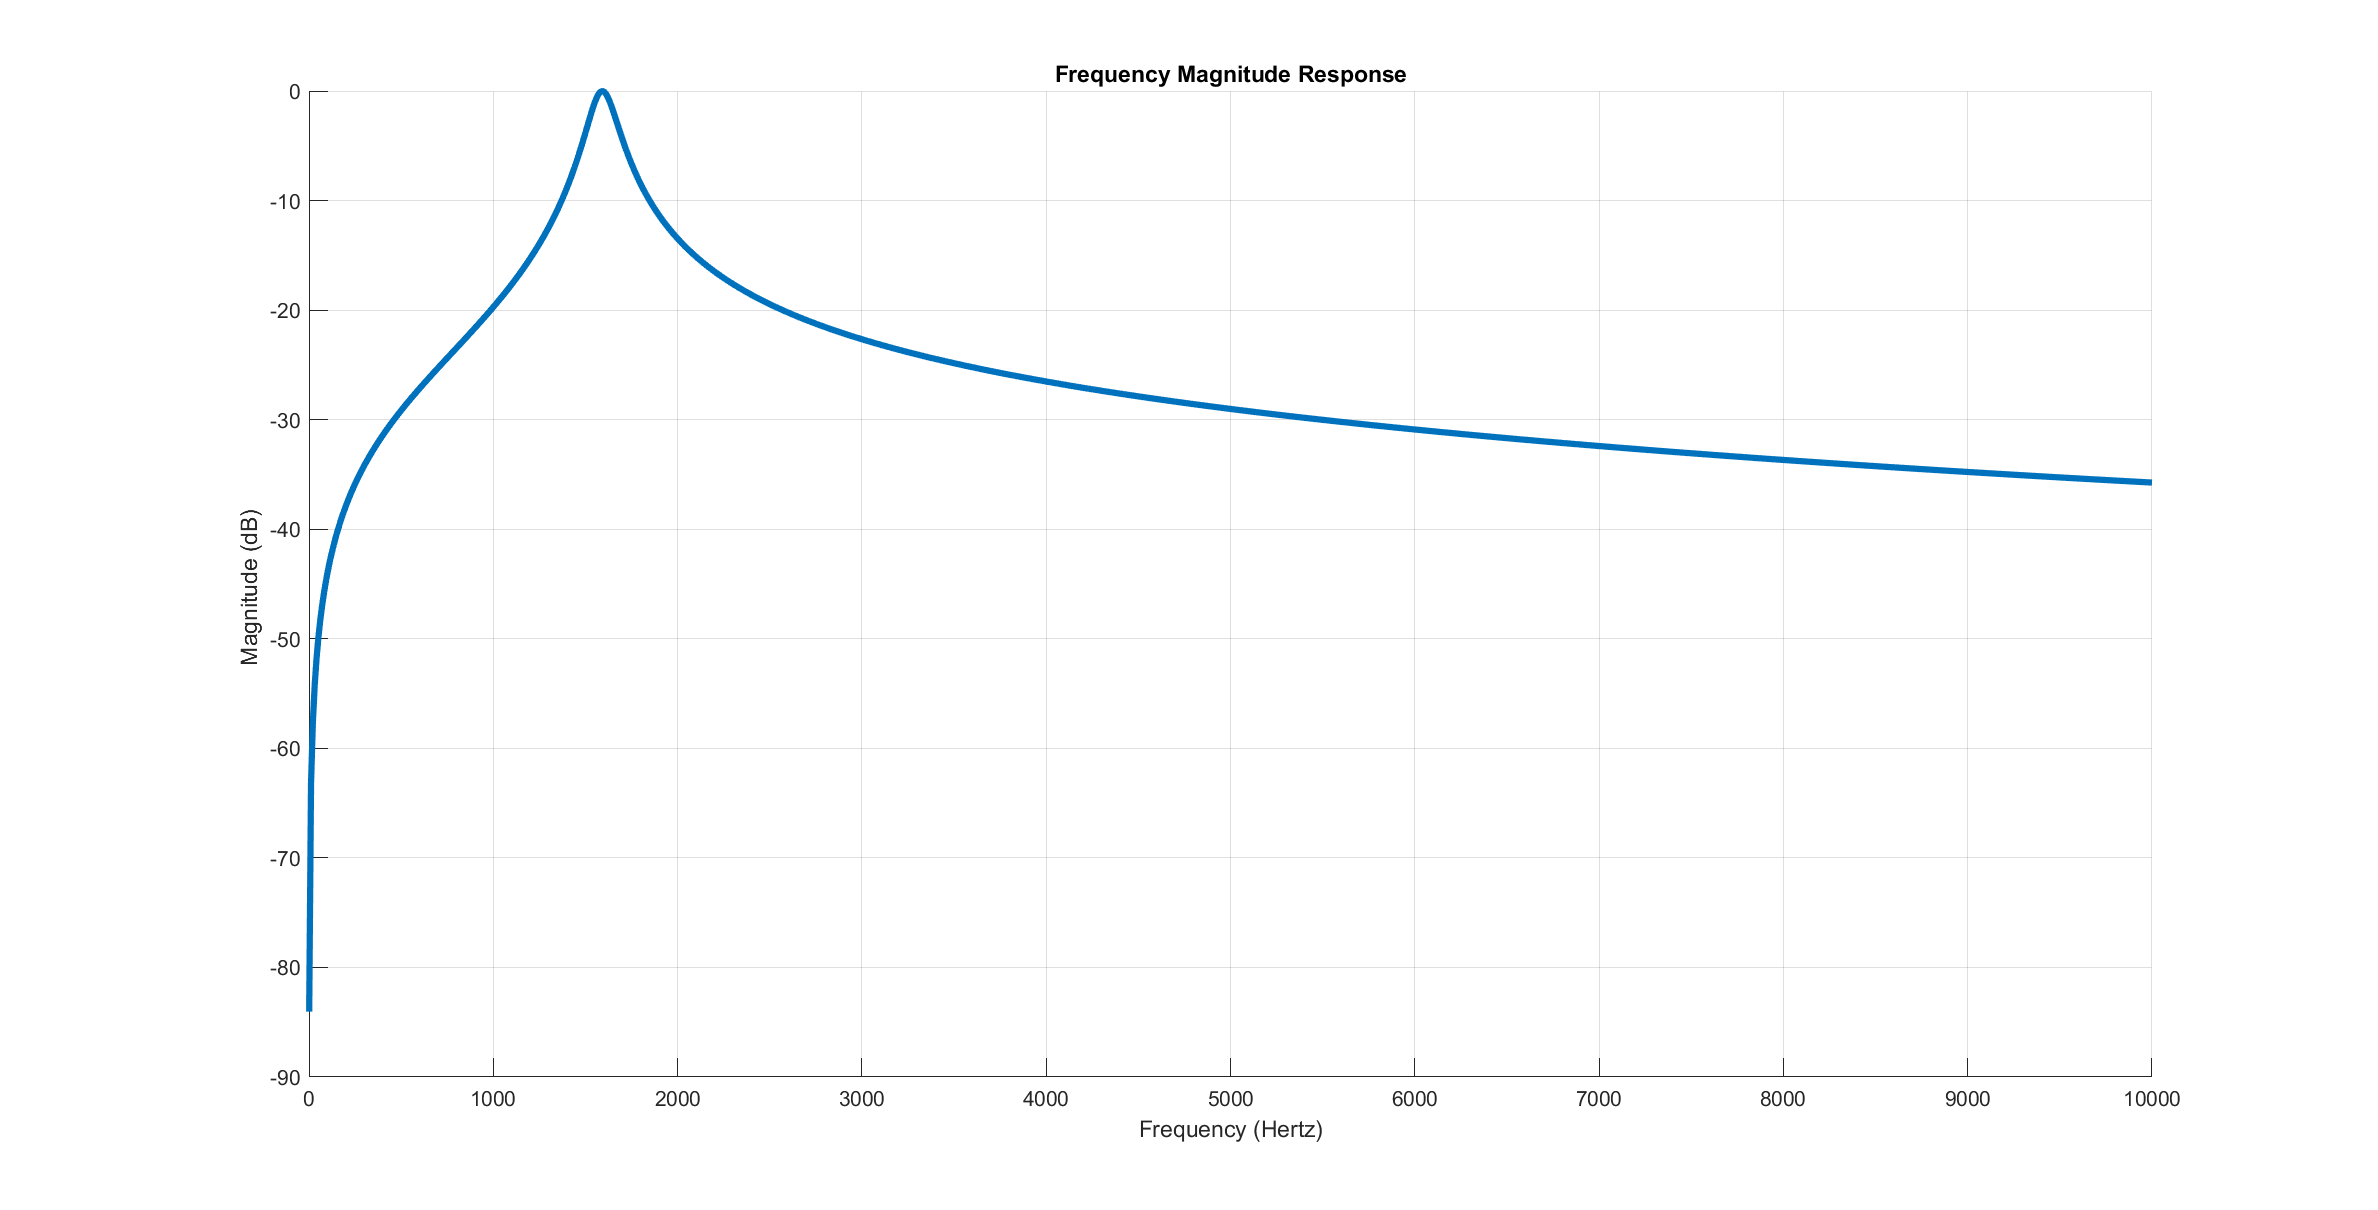
\includegraphics[width=1\textwidth]{6_3_2.png}
    \caption{Frequency Response of a Band Pass Filter}
\end{figure} 
\subsubsection{iii.}
Similarly for the square wave input with the response of our bandpass filter is obtained as given in Figure 13.
\begin{figure}[H]
    \centering
    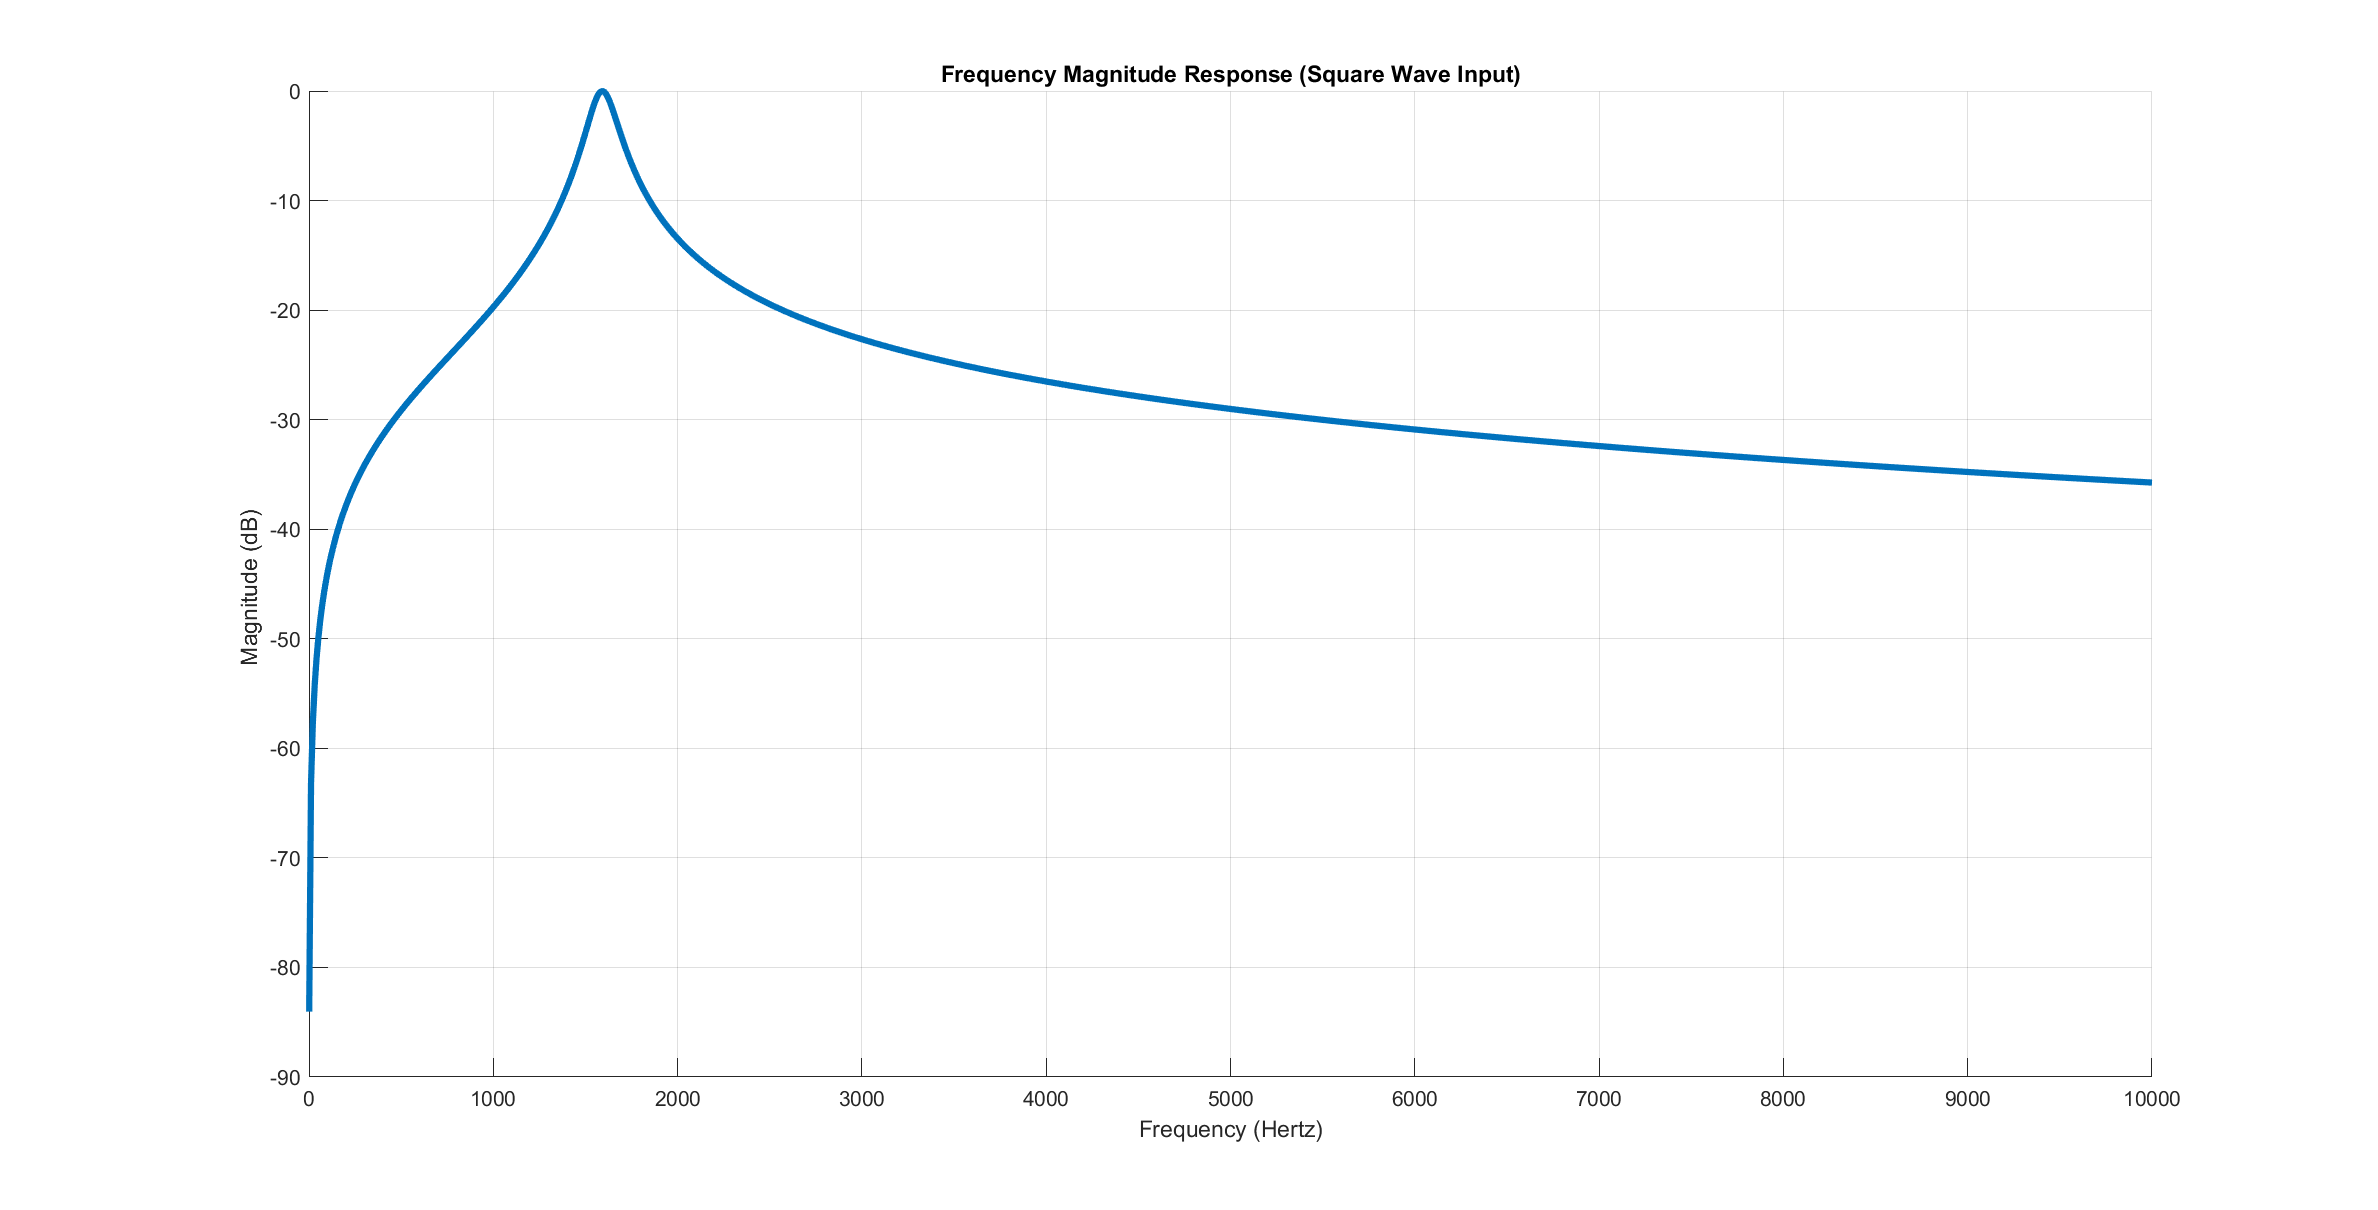
\includegraphics[width=1\textwidth]{6_3_3.png}
    \caption{Frequency Response of a Band Pass Filter (square wave input)}
\end{figure} 

\section{Conclusion}
In this preliminary document the characteristics of the filter topologies are investigated.
\section*{Appendix A}
The results of the some of the simulations are fetched from LTSpice and plotted in MATLAB in order to make the plots more readable and convenient.


\end{document}

%%%%%%%%%%%%%%%%%%%%%%   EXAMPLE TABLE   %%%%%%%%%%%%%%%%%%%%%%%%%%%%%%%%
\begin{table}[H]
\begin{center}
    \caption{Resistance reading by color code convention.}
    \vspace{2mm}
    \begin{tabular}{||c | c | c||} 
        \hline
        Color Order & Value & Tolerance \\ [0.5ex] 
        \hline\hline
        Brown / Black / Red / Gold & 1k\( \Omega \) & \( \% \) 5  \\ 
        \hline
        Yellow / Violet / Red / Gold & 4.7k\( \Omega \) & \( \% \) 5   \\
        \hline
        Brown / Grey / Orange / Gold & 18k\( \Omega \) & \( \% \) 5  \\ [1ex] 
        \hline
    \end{tabular}
\end{center}
\end{table}


%%%%%%%%%%%%%%%%%%%%%%   EXAMPLE IMAGE   %%%%%%%%%%%%%%%%%%%%%%%%%%%%%%%%
\begin{figure}[H]
\centering
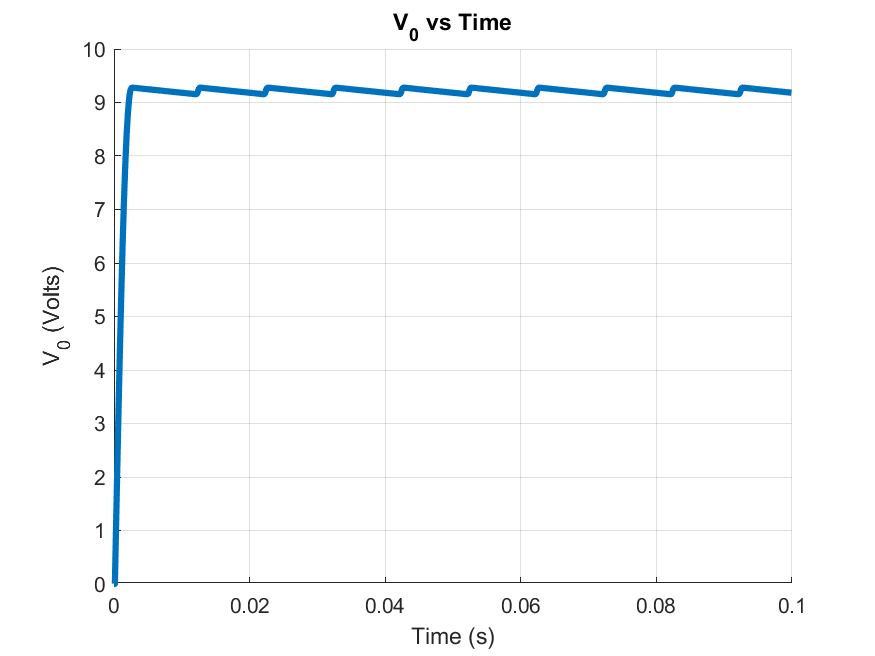
\includegraphics[width=1\textwidth]{5.png}
\caption{Circuit schematic for the step 5}
\end{figure} 

%%%%%%%%%%%%%%%%%%%%%%   EXAMPLE IMAGE FROM PDF   %%%%%%%%%%%%%%%%%%%%%%%%%%%%%%%%
\begin{figure}[H] \centering{
	\includegraphics[scale=0.25]{2a_plot.pdf}}
	\caption{Experiment 2}
\end{figure}
	